\lab{Абсолютный вольтметр}

\begin{lab:aim}
	установить количественное соотношение между единицами электрического напряжения в системах СИ и СГС.
\end{lab:aim}

\begin{lab:equipment}
	экспериментальный электростатический вольтметр, разновес, обычный электростатический вольтметр, выпрямитель, ключ.
\end{lab:equipment}

Измерив силу притяжения двух электродов, к которым приложено электрическое напряжение, можно определить величину этого
напряжения. На этом основан принцип действия электростатического вольтметра. Сила притяжения его электродов измеряется
путём сравнения с какой-нибудь механической силой, например с силой упругой деформации спиральной пружины. Так действуют
обычные электростатические вольтметры, широко применяемые в технике измерений. В данной работе электрическая сила
притяжения двух пластин плоского конденсатора сравнивается с весом гирек при помощи аналитических весов.

В системе СГС единица электрического заряда определяется через основные единицы: сантиметр, грамм и секунду. Поэтому,
измеряя одни только механические величины: силу притяжения электродов, их размеры и расстояние между ними,~--- можно
определить скопившийся на них заряд, а следовательно, и разность потенциалов между ними. Такие измерения и используемые
для этой цели приборы принято называть абсолютными.

В системе СИ вводится дополнительная основная единица силы тока~--- ампер. Единица электрического заряда определяется
через основные единицы: ампер и секунду. Как всегда в физике, введение добавочных независимых единиц приводит к
появлению размерных констант. В~формулах электростатики в системе СИ появляется размерная константа $\epsilon_0$, называемая
электрической постоянной. Определение этой константы является одной из задач данной работы.

Обозначим через $q$ заряд конденсатора и через $E_1$~--- напряжённость электрического поля, создаваемого одной из
пластин плоского конденсатора в том месте, где находится вторая пластина (считаем при этом, что расстояние $d$ между
пластинами мало по сравнению с поперечными размерами конденсатора). На вторую пластину действует со стороны первой сила
$F=qE_1$, равная, конечно, силе действия второй пластины на первую. Напряжённость поля $E_1$ связана с плотностью
электрического заряда $\sigma = q/S$ соотношением $E_1 = \sigma /2 \epsilon_0$. Таким образом,
\begin{equation}
	\eqmark{1}
	F=\frac{1}{2\epsilon_0}\frac{q^2}{S}.
\end{equation}
Для плоского конденсатора $q=UC=U \epsilon_0 S/d$, где $d$~--- расстояние между пластинами. Окончательно получаем
\begin{equation}
	\eqmark{2}
	F=\frac{\epsilon_0 SU^2}{2d^2},
\end{equation}
или
\begin{equation}
	\eqmark{3}
	U=d\sqrt{\frac{2F}{\epsilon_0 S}}\qquad(в~СИ).
\end{equation}

Формула \eqref{3} определяет в системе СИ связь между напряжением на конденсаторе и силой притяжения его пластин. Нетрудно
получить аналогичную формулу в системе СГС. Проводя те же рассуждения, что и выше, найдём
\begin{equation}
	\eqmark{4}
	U=2d\sqrt{\frac{2\pi F}{S}}\qquad(в~СГС).
\end{equation}

Опыты при постоянном напряжении на пластинах конденсатора можно использовать для определения электрической постоянной и
для измерения коэффициента, переводящего напряжение, выраженное в~вольтах, в единицы системы СГС. Квадратичный характер
связи между силой и напряжением позволяет измерять с~помощью весов и переменные напряжения, например напряжение
электрической сети. В нашей установке опыты проводятся только при постоянном напряжении.

%\fcpic[0.9]{1_2_1}{Схема экспериментальной установки}{1}
\begin{figure}
	\pic{0.9\textwidth}{1_2_1}
	\caption{Схема экспериментальной установки}
	\figmark{voltmeter-experiment}
\end{figure}

\experiment 

Основной составной частью экспериментальной установки являются аналитические весы (\figref{voltmeter-experiment}), одна из чашек которых
заменена подвижной пластиной~1 плоского воздушного конденсатора. Эта пластина заземлена. Высоковольтная неподвижная
пластина~2 помещена внутри заземлённого электростатического экрана~3. Верхняя часть экрана имеет вид кольца, окружающего
пластину~1 (охранное кольцо).

Нижние поверхности пластины и кольца лежат в одной плоскости. Так как их потенциалы равны, то они как бы образуют один
проводник; электрическое поле оказывается однородным вдоль всей поверхности подвижной пластины, в том числе и у её краев.

Напряжение на конденсатор подаётся от высоковольтного выпрямителя. Высокоомный резистор (3~МОм), вмонтированный в
выпрямитель, ограничивает ток короткого замыкания при случайных замыканиях пластин конденсатора. Параллельно пластинам
конденсатора включён обычный электростатический вольтметр.

%\rris{35mm}{1_2_2}{\cct Конструкция крепления подвижной пластины конденсатора}{2}
\begin{wrapfigure}{r}{0.4\textwidth}
	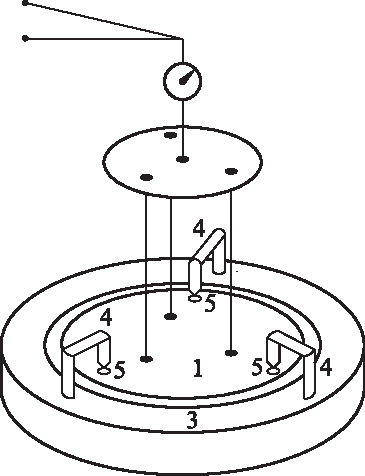
\includegraphics[width=0.38\textwidth]{1_2_2}
	\caption{Конструкция крепления подвижной пластины конденсатора}
	\figmark{voltmeter-capacitor}
\end{wrapfigure}

Измерения проводятся в условиях равновесия электрических и механических сил. Как следует из формулы (\eqref{2}),
электрические силы быстро возрастают с уменьшением зазора между пластинами. С другой стороны, механические силы,
обеспечивающие равновесие аналитических весов, возрастают при наклонах коромысла крайне медленно. В условиях нашего
опыта равновесие весов при равенстве электрических и механических сил оказывается поэтому неустойчивым.

При настройке прибора на левую чашку весов кладётся некоторый перегрузок. При этом положение весов фиксируется тремя
контактными винтами 4, расположенными в~вершинах равностороннего треугольника (\figref{voltmeter-experiment} и \eqref{2}). Винты упираются в
контактные площадки 5, установленные на верхней плоскости подвижной пластины. Напряжение на пластинах регулируется с
помощью реостата $R$ выпрямителя. Электрические силы, действующие на пластину 1, возрастают по мере увеличения
потенциала неподвижной пластины. В тот момент, когда эти силы сравниваются с~весом перегрузка, коромысло теряет
устойчивость и подвижная пластина <<прилипает>> к неподвижной. Этот момент фиксируется по движению стрелки весов.

\begin{lab:task}
	
	В работе предлагается исследовать связь между силой  притяжения пластин и разностью потенциалов между ними для
	определения электрической постоянной $\epsilon_0$ и коэффициента перевода единиц напряжения из системы СГС в систему СИ.
	
	\warning{Регулировка измерительного конденсатора требует определённых навыков и может производиться \important{только
	лаборантом или механиком}. Студент проверяет регулировку пластин визуально, не меняя их настройку самостоятельно.}
	
	\begin{enumerate}
		\item Перед началом работы рассчитайте по формуле (\eqref{2}) максимально допустимую нагрузку, исходя из предела измерений
		электростатического вольтметра. Расстояние между пластинами~$d$ и площадь пластин~$S$ указаны на установке.
		
		\item Соберите схему согласно Рис.~\figref{voltmeter-experiment}.
		
		По уровню, расположенному на основании весов, проверьте, занимает ли платформа весов горизонтальное положение. При этом
		подвижная пластина измерительного конденсатора должна располагаться в~центре охранного кольца, не касаясь его. При
		обнаружении неисправностей обратитесь к лаборанту.
		
		Проверьте регулировку положения равновесия коромысла ненагруженных весов. Для этого следует отключить пластины
		конденсатора от выпрямителя и соединить их друг с другом (ключ К на Рис.~\figref{voltmeter-experiment} переводится в нижнее положение). Осторожно,
		чтобы не сбить опорные призмы коромысла, освободите весы от арретира. В положении равновесия при закороченных пластинах
		упорные штифты должны быть близки к контактным пластинам и должны касаться их при незначительных ($\sim 10$~мг)
		перегрузках на левой чашке весов.
		
		При необходимости проведите регулировку положения коромысла весов. Для этого снова арретируйте весы и, перемещая
		тарировочные гайки, расположенные на концах коромысла, добейтесь того, чтобы стрелка весов оказалась на нулевом делении
		шкалы. Поворот гаек и изменение груза на чашке весов \important{всегда производятся при арретированных весах}, а проверка
		положения коромысла~--- когда весы сняты с арретира. Для изменения груза открываются боковые дверцы весов (фронтальная
		дверца открывается только на время ремонта).
		
		\item Исследуйте зависимость силы притяжения пластин от напряжения на конденсаторе. Для измерения напряжения применяется
		электростатический вольтметр (вольтметр, вмонтированный в выпрямитель, для измерений не используется).
		
		Переведите ключ К в положение измерения. Положите на левую чашку весов груз, равный примерно 0,1 от максимально
		допустимого. При этом подвижная пластина должна прижаться к упорным штифтам. Подберите напряжение, приводящее к потере
		устойчивости весов. Оно соответствует моменту начала движения стрелки весов.
		
		Рекомендуется уточнить это напряжение 2--3 раза, каждый раз всё медленнее поворачивая ручку реостата $R$. Перед каждым
		измерением напряжения следует закорачивать пластины конденсатора ключом К, чтобы снять с пластин остаточный заряд.
		
		Проведите такие измерения не менее чем в десяти точках, равномерно расположенных в рабочем диапазоне нагрузок.
		
		\item Сразу после измерений изобразите результаты на графике в координатах $F$, $U^2$. Если полученные точки в пределах
		ошибок опыта ложатся на прямую линию, эксперимент можно закончить. Если прямой линии не получилось, следует найти и
		устранить ошибку.
		
		\item По наклону прямой $F=f(U^2)$  рассчитайте значение электрической постоянной $\epsilon_0$.
		
		\item Используйте результаты измерений для определения коэффициента перевода единиц напряжения из системы СГС в систему СИ.
		Напряжение в единицах СГС может быть вычислено по формуле (\eqref{4}), а показания электростатического вольтметра позволяют
		определить это напряжение в вольтах. Изобразите полученные результаты на графике в координатах $U$~(в~СГС)$=f(U,~В)$ и по
		наклону прямой, проведённой через экспериментальные точки, определите коэффициент пересчёта напряжений.

	\end{enumerate}

\end{lab:task}

\begin{lab:questions}
	\item Оцените ошибку, возникающую вследствие того, что равновесие весов устанавливалось при наличии небольшого зазора между
	штифтами и контактными пластинами, а измерения производятся при отсутствии этого зазора.
	
	\item Покажите, что электростатический вольтметр пригоден для измерения как постоянного, так и переменного напряжения.
	
	\item Покажите, что измерения на переменном токе определяют именно эффективное значение его напряжения.
	
	\item Чем определяется интервал частот, в котором можно измерять переменные напряжения с помощью электростатического
	вольтметра?
\end{lab:questions}

\begin{lab:literature}
	\item {\em Сивухин Д.В.} Общий курс физики. Т.~III. Электричество --- М.: Наука, 1983, \S~125.
	
	\item {\em Калашников С.Г.} Электричество.~--- М.: Наука, 1977, \S\S~5, 6, 26.
	
	%\item {\em Кингсеп А.С., Локшин Г.Р., Ольхов О.А.} Основы физики. Т.~1. Ч.~III. Электричество и магнетизм.~--- М.:
	%Физматлит, 2001.
\end{lab:literature}

